% CS615 Aspects of System Administration
% Author: Jan Schaumann <jschauma@netmeister.org>
% $Id: slides.tex,v 1.6 2006/03/07 13:55:55 jschauma Exp $

\documentclass[xga]{xdvislides}
\usepackage[landscape]{geometry}
\usepackage{graphics}
\usepackage{graphicx}
\usepackage{colordvi}

\begin{document}
\setfontphv

%%% Headers and footers
\lhead{\slidetitle}                               % default:\lhead{\slidetitle}
\chead{CS615 - Aspects of System Administration}% default:\chead{\relax}
\rhead{Slide \thepage}                       % default:\rhead{\sectiontitle}
\lfoot{\Gray{Automation Part II / Backup and Disaster Recovery}}% default:\lfoot{\slideauthor}
\cfoot{\relax}                               % default:\cfoot{\relax}
\rfoot{\Gray{\today}}

\vspace*{\fill}
\begin{center}
	\Hugesize
		CS615 - Aspects of System Administration\\ [1em]
		Automation Part II \\ [1em]
		Backup and Disaster Recovery \\ [1em]
	\hspace*{5mm}\blueline\\ [1em]
	\Normalsize
		Department of Computer Science\\
		Stevens Institute of Technology\\
		Jan Schaumann\\
		\verb+jschauma@stevens-tech.edu+
		\verb+http://www.cs.stevens-tech.edu/~jschauma/615A/+
\end{center}
\vspace*{\fill}

\newpage
\vspace*{\fill}
\begin{center}
    \Hugesize
        Hooray! \\ [1em]
    \hspace*{5mm}
    \blueline\\
    \hspace*{5mm}\\
        5 Minute Break
\end{center}
\vspace*{\fill}

\subsection{Regular Expressions}
A regular expression is a pattern that describes a set of strings. \\

\begin{itemize}
	\item patterns can be a combination of
		\begin{itemize}
			\item a fixed string (\verb+abc+)
		\end{itemize}
\end{itemize}
\vspace{.5in}
\begin{verbatim}
$ ifconfig -a | egrep "inet"
\end{verbatim}

\subsection{Regular Expressions}
A regular expression is a pattern that describes a set of strings. \\

\begin{itemize}
	\item patterns can be a combination of
		\begin{itemize}
			\item a fixed string (\verb+abc+)
			\item a bracket expression, such as
				\begin{itemize}
					\item a number of characters -- \verb+[aK2l,]+
				\end{itemize}
		\end{itemize}
\end{itemize}
\vspace{.5in}
\begin{verbatim}
$ ifconfig -a | egrep "[UBS]"
\end{verbatim}

\subsection{Regular Expressions}
A regular expression is a pattern that describes a set of strings. \\

\begin{itemize}
	\item patterns can be a combination of
		\begin{itemize}
			\item a fixed string (\verb+abc+)
			\item a bracket expression, such as
				\begin{itemize}
					\item a number of characters -- \verb+[aK2l,]+
					\item a range expression -- \verb+[a-z]+
				\end{itemize}
		\end{itemize}
\end{itemize}
\vspace{.5in}
\begin{verbatim}
$ ifconfig -a | egrep "[A-Z]"
\end{verbatim}



\subsection{Regular Expressions}
A regular expression is a pattern that describes a set of strings. \\

\begin{itemize}
	\item patterns can be a combination of
		\begin{itemize}
			\item a fixed string (\verb+abc+)
			\item a bracket expression, such as
				\begin{itemize}
					\item a number of characters -- \verb+[aK2l,]+
					\item a range expression -- \verb+[a-z]+
					\item a negated bracket expression -- \verb+[^0-9]+
				\end{itemize}
		\end{itemize}
\end{itemize}
\vspace{.5in}
\begin{verbatim}
$ ifconfig -a | egrep "[^a-zA-Z0-9      <>%,:.()]"
\end{verbatim}



\subsection{Regular Expressions}
A regular expression is a pattern that describes a set of strings. \\

\begin{itemize}
	\item patterns can be a combination of
		\begin{itemize}
			\item a fixed string (\verb+abc+)
			\item a bracket expression, such as
				\begin{itemize}
					\item a number of characters -- \verb+[aK2l,]+
					\item a range expression -- \verb+[a-z]+
					\item a negated bracket expression -- \verb+[^0-9]+
				\end{itemize}
			\item a character with a special meaning, such as
				\begin{itemize}
					\item \verb+.+ -- any single character
				\end{itemize}
		\end{itemize}
\end{itemize}
\vspace{.5in}
\begin{verbatim}
$ ifconfig -a | egrep "flags."
\end{verbatim}



\subsection{Regular Expressions}
A regular expression is a pattern that describes a set of strings. \\

\begin{itemize}
	\item patterns can be a combination of
		\begin{itemize}
			\item a fixed string (\verb+abc+)
			\item a bracket expression, such as
				\begin{itemize}
					\item a number of characters -- \verb+[aK2l,]+
					\item a range expression -- \verb+[a-z]+
					\item a negated bracket expression -- \verb+[^0-9]+
				\end{itemize}
			\item a character with a special meaning, such as
				\begin{itemize}
					\item \verb+.+ -- any single character
					\item \verb+^+ -- beginning of line
					\item \verb+$+ -- end of line
				\end{itemize}
		\end{itemize}
\end{itemize}
\vspace{.5in}
\begin{verbatim}
$ ifconfig -a | egrep "[0-9]$"
\end{verbatim}

\subsection{Regular Expressions}
\begin{itemize}
	\item patterns can be followed by qualifiers and quantifiers
		\begin{itemize}
			\item \verb+?+ -- the pattern is optional and matched at most once
			\item \verb+*+ -- the pattern will be matched zero or more times
			\item \verb|+| -- the pattern will be matched one or more times
			\item \verb+{n}+ -- the pattern is matched exactly \verb+n+ times
			\item \verb+{n,}+ -- the pattern is matched \verb+n+ or more times
			\item \verb+{n,m}+ -- the pattern is matched at least \verb+n+,
				but no more than \verb+m+ times
		\end{itemize}
	\item patterns can be logically grouped together \verb+(1[a-z]2|a[0-9]z)+
	\item matched patterns can be remembered and referenced lateron
\end{itemize}

\subsection{Regular Expressions}
Identify all network interfaces:
\begin{verbatim}
$ ifconfig -a | sed -n -E 's/^([a-z]+[0-9]).*/\1/p'
$ ifconfig -a | sed -n -E 's/^([a-z]+(([0-9]+)|:[0-9]+)?).*/\1/p'
\end{verbatim}
\vspace{.5in}
Now you:
\begin{itemize}
	\item extract all IP addresses
	\item extract all MAC addresses
	\item extract all netmasks
\end{itemize}

\subsection{Remember to use the right tool for the job}
Bourne shell ({\tt /bin/sh}):
\begin{itemize}
	\item lowest common denominator
	\item available and reliable on most platforms (but beware of
		non-portable {\tt bash(1)} ``enhancements'')
	\item beware of ``quick-and-dirty'' solutions, they grow to become
		unmaintainable
	\item treat shell as any other programming language:
		\begin{itemize}
			\item use functions
			\item use suitably scoped variables
			\item follow Unix philosophy
			\item properly package your tool
		\end{itemize}
\end{itemize}

\subsection{Remember to use the right tool for the job}
Perl, Python, Ruby, ...
\begin{itemize}
	\item suitable for moderately complex tasks
	\item move to these when {\tt sed(1)}, {\tt awk(1)} and friends
		become too cumbersome
	\item text manipulation frequently ``easier'' in perl
	\item beware of ``quick-and-dirty'' solutions, they grow to become
		unmaintainable
	\item try to build self-contained {\em modules} that can be tested
		independent of the ``main'' program
	\item wealth of libraries available
		\begin{itemize}
			\item use them!
			\item remember to explicitly {\em require} them
				(dependencies)
		\end{itemize}
	\item properly package your tool
\end{itemize}

\subsection{Remember to use the right tool for the job}
Perl, Python, PHP, Ruby, JavaScript, ...
\begin{itemize}
	\item http/web server interfaces
	\item CGI ``scripts''
	\item server-side execution
	\item interface with/utilize APIs in a specific domain/vendor products
	\item frequent cause of all sorts of security problems due to
		interface with user data / exposure on the internet
\end{itemize}

\subsection{Remember to use the right tool for the job}
Java, Scala, Clojure, ...
\begin{itemize}
	\item know your primary applications
	\item interface with / extend / tie into JVM
\end{itemize}
\vspace{.5in}
C, C++, Go, ...
\begin{itemize}
	\item performance benefits
	\item portability
	\item sufficient low-levelness
	\item systems understanding
	\item fix/patch your tools
\end{itemize}

\subsection{Of course...}
\vspace*{\fill}
\begin{center}
	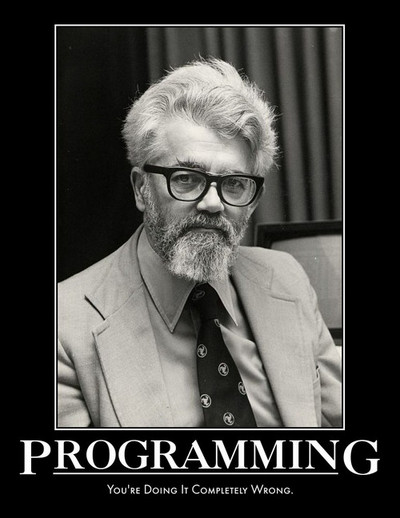
\includegraphics[scale=0.65]{pics/WrongProgramming.eps}
\end{center}
\vspace*{\fill}


\subsection{Scripting / interpreted Languages}
General advantages:
\begin{itemize}
	\item short development cycle
	\item normally facilitates things like string manipulation,
		arithmetic and more complex regular expressions
	\item easily handles multiple file handles and other I/O
	\item some security features
	\item tens of thousands of special- and general-purpose modules
		available
\end{itemize}

\subsection{Scripting / interpreted Languages}
General disadvantages:
\begin{itemize}
	\item no one tool fits all purposes
	\item tens of thousands of special- and general-purpose modules
		available $\rightarrow$ lots of duplication, stale code,
		questionable quality
	\item security features frequently neglected or circumvented ("too
		hard" / "inconvenient")
	\item everybody has their particular favorite (and dislikes one or
		the other)
	\item interpreter not (necessarily) universally available /
		installed
\end{itemize}

\subsection{User Interface}
\\
\vspace*{\fill}
\begin{center}
	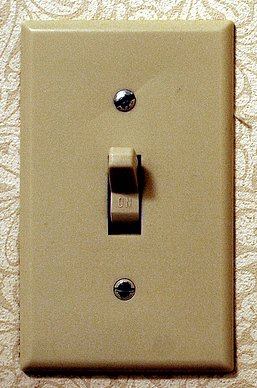
\includegraphics[scale=3]{pics/switch.eps}
\end{center}
\vspace*{\fill}

\subsection{Unix Philosophy}
\\
\Huge
\begin{center}
	Write programs that do one thing and do it well.\\
	\vspace{.5in}
	Write programs to work together. \\
	\vspace{.5in}
	Write programs to handle text streams, because that is a universal interface.
\end{center}
\Normalsize

\subsection{The KISS Principle}
\\
\vspace*{\fill}
\begin{center}
	
\includegraphics[scale=0.3]{pics/kiss.eps}
\end{center}
\vspace*{\fill}

\subsection{POLA}
Principle of Least Astonishment
\\
\vspace*{\fill}
\begin{center}
	
\includegraphics[scale=0.7]{pics/kinder-surprise.eps}
\end{center}
\vspace*{\fill}

\subsection{Test Driven}
\vspace*{\fill}
\begin{center}
	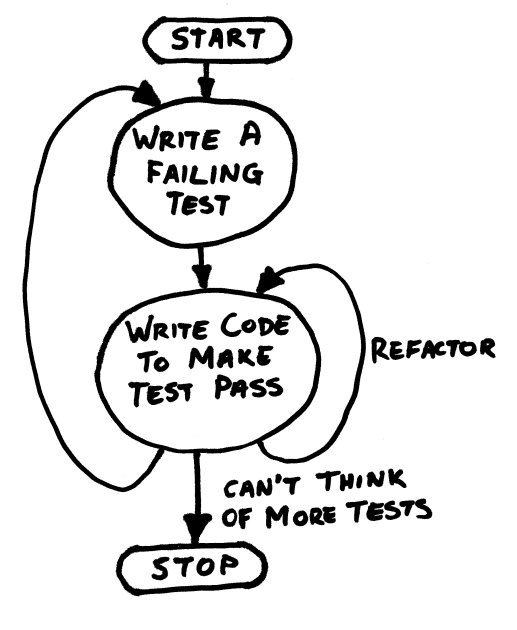
\includegraphics[scale=2.0]{pics/tdd.eps}
\end{center}
\vspace*{\fill}

\subsection{Avoid the Quick Fix}
\\
\Huge
\begin{center}
	There's nothing as permanent as a temporary solution.
\end{center}
\Normalsize

\subsection{Take a good look in the mirror!}
\\
\vspace*{\fill}
\begin{center}
	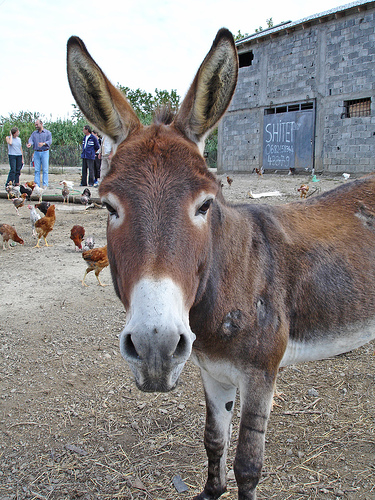
\includegraphics[scale=0.65]{pics/donkey.eps} \\
	\small
	Nice Ass!
\end{center}
\vspace*{\fill}

\subsection{Take a good look in the mirror!}
\\
\Huge
\begin{center}
	Until you can {\em prove} otherwise, \\
	assume that {\em you} are the Ass!
\end{center}
\Normalsize

\subsection{Avoid the Project That Was Never Finished}
\\
\Huge
\begin{center}
	Don't let the Perfect be the enemy of the Good.
\end{center}
\Normalsize

\subsection{Avoid Feature Creep}
\vspace*{\fill}
\begin{center}
	
\includegraphics[scale=1.0]{pics/feeping.eps} \\
	\small
	\verb+http://www.feepingcreatures.com+
\end{center}
\vspace*{\fill}

\subsection{Release Early, Release Often}
\\
\Huge
\begin{center}
	``More users find more bugs.'' \\
	\addvspace{.2in}
	\small F. Brooks, ``The Mythical Man Month''
\end{center}
\Normalsize

\subsection{Increase the Bus Factor}
\vspace*{\fill}
\begin{center}
	\includegraphics[scale=0.85]{pics/bert-ernie.eps} \\
	\small
	``Just friends.''
\end{center}
\vspace*{\fill}

\subsection{Fix Broken Windows}
\vspace*{\fill}
\begin{center}
	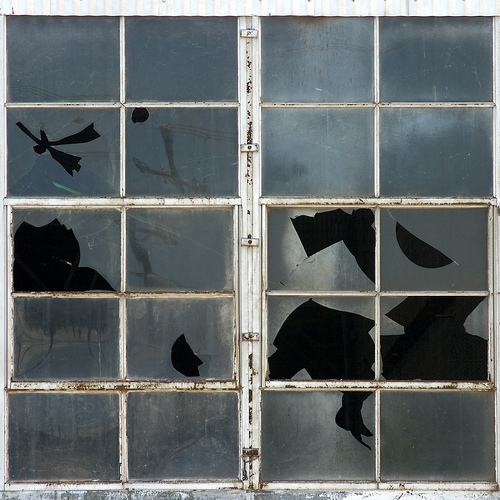
\includegraphics[scale=0.6]{pics/broken-windows.eps}
\end{center}
\vspace*{\fill}

\subsection{Program Maintenance}
\\
\Huge
\begin{center}
	``... is an entropy-increasing process, and even its most skillful
	execution only delays the subsidence of the system into unfixable
	obsolescence.'' \\
	\addvspace{.2in}
	\small F. Brooks, ``The Mythical Man Month''
\end{center}
\Normalsize

\subsection{Toss it!}
\vspace*{\fill}
\begin{center}
	
\includegraphics[scale=3]{pics/waste.eps}
\end{center}
\vspace*{\fill}

\subsection{Starting fresh}
\vspace*{\fill}
\begin{center}
	
\includegraphics[scale=2]{pics/clean-slate.eps}
\end{center}
\vspace*{\fill}

\newpage
\vspace*{\fill}
\begin{center}
    \Hugesize
        Hooray! \\ [1em]
    \hspace*{5mm}
    \blueline\\
    \hspace*{5mm}\\
        5 Minute Break
\end{center}
\vspace*{\fill}

\subsection{And now for something completely different...}
\begin{itemize}
	\item backup vs. restore
\end{itemize}

\subsection{And now for something completely different...}
\begin{itemize}
	\item backup vs. restore
	\item backup devices and media
\end{itemize}
\vspace*{\fill}
\begin{center}
	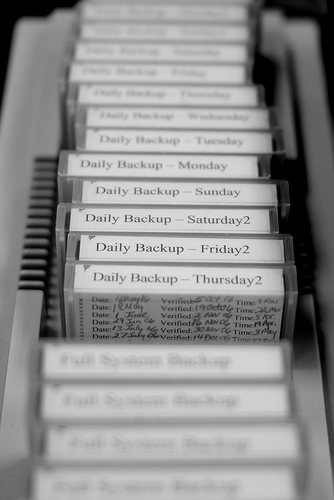
\includegraphics[scale=2.0]{pics/daily-tapes.eps}
\end{center}
\vspace*{\fill}

\subsection{And now for something completely different...}
\begin{itemize}
	\item backup vs. restore
	\item backup devices and media
\end{itemize}
\vspace*{\fill}
\begin{center}
	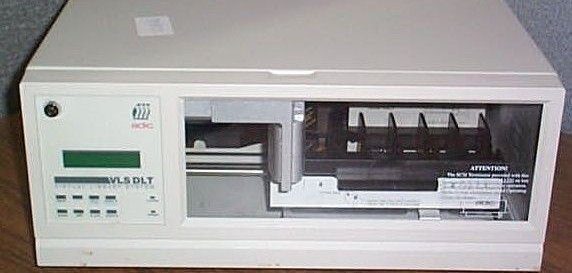
\includegraphics[scale=0.8]{pics/dlt-library.eps}
\end{center}
\vspace*{\fill}

\subsection{And now for something completely different...}
\begin{itemize}
	\item backup vs. restore
	\item backup devices and media
\end{itemize}
\vspace*{\fill}
\begin{center}
	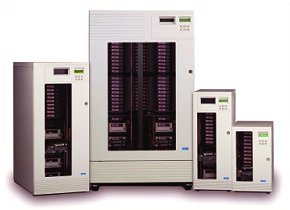
\includegraphics[scale=1.0]{pics/libraries.eps}
\end{center}
\vspace*{\fill}

\subsection{And now for something completely different...}
\begin{itemize}
	\item backup vs. restore
	\item backup devices and media
	\item filesystem considerations
\end{itemize}

\subsection{And now for something completely different...}
\begin{itemize}
	\item backup vs. restore
	\item backup devices and media
	\item filesystem considerations
	\item backup strategies
\end{itemize}

\subsection{And now for something completely different...}
\begin{itemize}
	\item backup vs. restore
	\item backup devices and media
	\item filesystem considerations
	\item backup strategies
	\item planning for disasters
\end{itemize}

\subsection{Backups and Restore Basics}
Why are backups needed?

\subsection{Backups and Restore Basics}
Why are backups needed?
\begin{itemize}
	\item off-site storage of sensitive data
	\item long-term data storage
	\item data loss
\end{itemize}

\subsection{Backups and Restore Basics}
Why are backups needed?
\begin{itemize}
	\item off-site storage of sensitive data
	\item long-term data storage
	\item data loss due to
\end{itemize}
\vspace*{\fill}
\begin{center}
	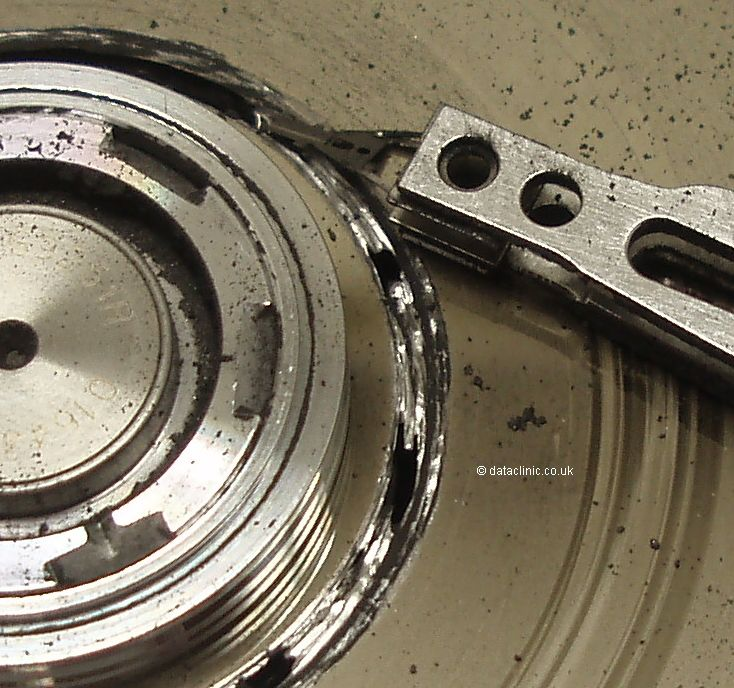
\includegraphics[scale=1.0]{pics/headcrash-closeup.eps}
\end{center}
\vspace*{\fill}

\subsection{Backups and Restore Basics}
Why are backups needed?
\begin{itemize}
	\item off-site storage of sensitive data
	\item long-term data storage
	\item data loss due to
\end{itemize}
\vspace*{\fill}
\begin{center}
	
\includegraphics[scale=1.2]{pics/dumb-user.eps}
\end{center}
\vspace*{\fill}

\subsection{Backups and Restore Basics}
Why are backups needed?
\begin{itemize}
	\item off-site storage of sensitive data
	\item long-term data storage
	\item data loss due to
\end{itemize}
\vspace*{\fill}
\begin{center}
	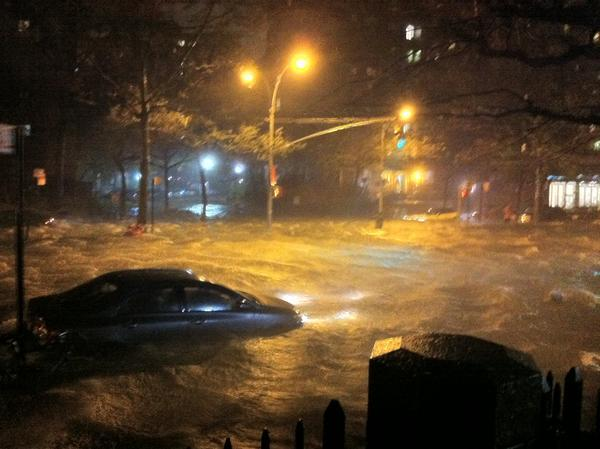
\includegraphics[scale=0.4]{pics/20th-and-C.eps}
\end{center}
\vspace*{\fill}

\subsection{Backups and Restore Basics}
Why are backups needed?
\begin{itemize}
	\item off-site storage of sensitive data
	\item long-term data storage
	\item data loss due to
\end{itemize}
\vspace*{\fill}
\begin{center}
	
\includegraphics[scale=0.6]{pics/hacker.eps}
\end{center}
\vspace*{\fill}

\subsection{Backups and Restore Basics}
Why are backups needed?
\begin{itemize}
	\item off-site storage of sensitive data
	\item long-term data storage
	\item data loss due to
\end{itemize}
\vspace*{\fill}
\begin{center}
	
\includegraphics[scale=0.6]{pics/bugs.eps}
\end{center}
\vspace*{\fill}

\subsection{Backups and Restore Basics}
Why are backups needed?
\begin{itemize}
	\item off-site storage of sensitive data
	\item long-term data storage
	\item data loss due to
		\begin{itemize}
			\item equipment failure
			\item bozotic users
			\item natural disaster
			\item security breach
			\item software bugs
		\end{itemize}
\end{itemize}

\subsection{Backups and Restore Basics}
Why are backups needed?
\begin{itemize}
	\item off-site storage of sensitive data
	\item long-term data storage
	\item data loss due to
		\begin{itemize}
			\item equipment failure
			\item bozotic users
			\item natural disaster
			\item security breach
			\item software bugs
		\end{itemize}
\end{itemize}
\addvspace{.5in}
Think of your backups as {\em insurance}:  you invest and pay for it, hoping
you will never need it.


\subsection{Key Reasons for Restores}
Three key reasons for restores: {\em Accidental File Deletion}, {\em Disk
Failure} and {\em Archival}.
\\

1. Accidental File Deletion
\begin{itemize}
	\item ability to restore a file within a certain time frame
	\item restore time, including
		\begin{itemize}
			\item actual time spent restoring
			\item waiting until resources permit the restore
			\item staff availability
		\end{itemize}
	\item self-service restore
\end{itemize}

\subsection{Key Reasons for Restores}
2. Disk Failure
\begin{itemize}
	\item loss of entire file system
	\item leads to downtime
	\item RAID may help
	\item takes long time to restore
\end{itemize}
\addvspace{.5in}
3. Archival
\begin{itemize}
	\item {\em full} set of level 0 backups
	\item separate set from regular backups
	\item usually stored off-site
	\item store for long time
\end{itemize}

\subsection{Filesystem backup}
\vspace*{\fill}
\begin{center}
	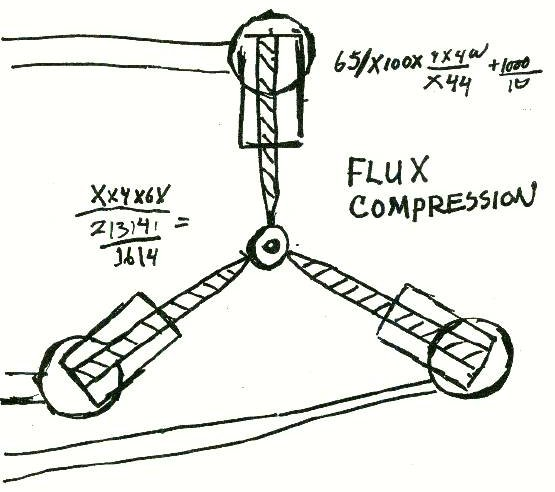
\includegraphics[scale=0.7]{pics/flux-capacitor.eps}
\end{center}
\vspace*{\fill}

\subsection{Filesystem backup}
\vspace*{\fill}
\begin{center}
	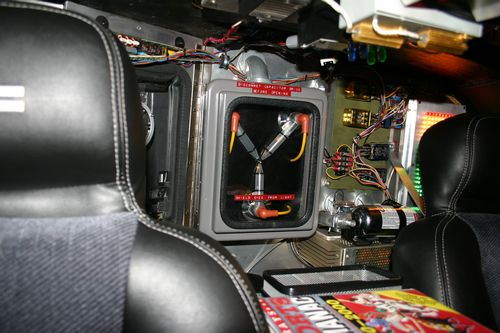
\includegraphics[scale=2.5]{pics/flux-capacitor2.eps}
\end{center}
\vspace*{\fill}

\subsection{Filesystem backup}
\vspace*{\fill}
\begin{center}
	
\includegraphics[scale=0.6]{pics/Time_Machine.eps}
\end{center}
\vspace*{\fill}


\subsection{Filesystem backup}
Example: Mac OS X ``Time Machine'':
\begin{itemize}
	\item automatically creates a full backup (equivalent of a "level 0 dump")
		to separate device or NAS, recording (specifically) last-modified date
		of all directories
	\item every hour, creates a full copy via {\em hardlinks} (hence no
		additional disk space consumed) for files that have not changed,
		new copy of files that have changed
		\item changed files are determined by inspecting last-modified date of
			directories (cheaper than doing comparison of all files'
			last-modified date or data)
	\item saves hourly backups for 24 hours, daily backups for
		the past month, and weekly backups for everything older than a month.
\end{itemize}

\subsection{Filesystem backup}
\vspace*{\fill}
\begin{center}
	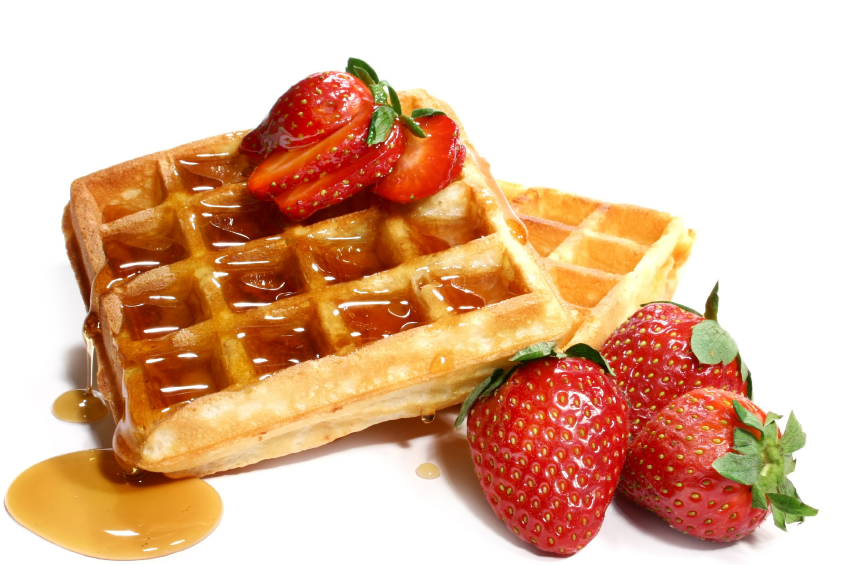
\includegraphics[scale=1.0]{pics/waffles.eps}
\end{center}
\vspace*{\fill}


\subsection{Filesystem backup}
Example: WAFL (Write Anywhere File Layout)
\begin{itemize}
	\item used by NetApp's ``Data ONTAP'' OS
	\item a snapshot is a read-only copy of a file system (cheap and near
		instantaneous, due to CoW)
	\item uses regular snapshots (``consistency points'', every 10 seconds)
		to allow for speedy recovery from crashes
\end{itemize}

\subsection{Filesystem backup}
Example: WAFL (Write Anywhere File Layout)
\vspace*{\fill}
\begin{center}
	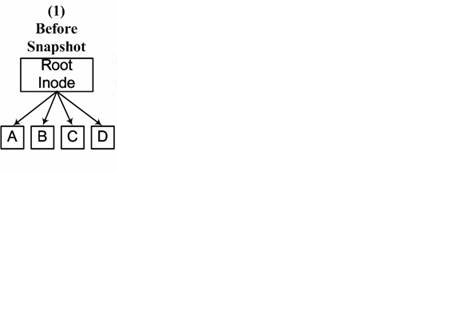
\includegraphics[scale=1.0]{pics/wafl0.eps}
\end{center}
\vspace*{\fill}


\subsection{Filesystem backup}
Example: WAFL (Write Anywhere File Layout)
\vspace*{\fill}
\begin{center}
	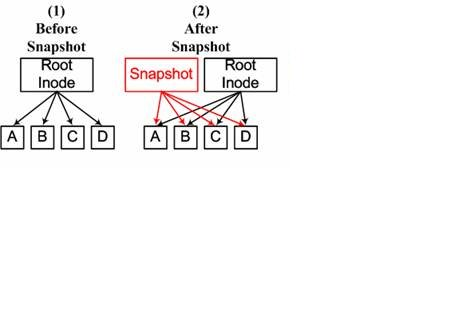
\includegraphics[scale=1.0]{pics/wafl1.eps}
\end{center}
\vspace*{\fill}


\subsection{Filesystem backup}
Example: WAFL (Write Anywhere File Layout)
\vspace*{\fill}
\begin{center}
	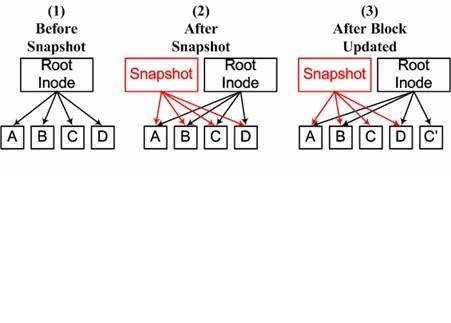
\includegraphics[scale=1.0]{pics/wafl2.eps}
\end{center}
\vspace*{\fill}


\subsection{Filesystem backup}
Example: WAFL (Write Anywhere File Layout)
\vspace*{\fill}
\begin{center}
	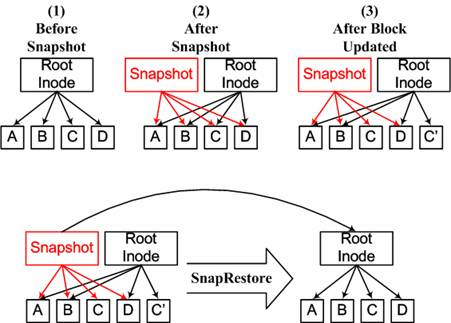
\includegraphics[scale=1.0]{pics/wafl.eps}
\end{center}
\vspace*{\fill}


\subsection{Filesystem backup}
Example: ZFS snapshots
\begin{itemize}
	\item ZFS uses a copy-on-write transactional object model (new data does
		not overwrite existing data, instead modifications are written to a
		new location with existing data being referenced), similar to WAFL
	\item a snapshot is a read-only copy of a file system (cheap and near
		instantaneous, due to CoW)
	\item initially consumes no additional disk space; the writable filesystem
		is made available as a ``clone''
	\item conceptually provides a branched view of the filesystem; normally
		only the ``active'' filesystem is writable
\end{itemize}

\subsection{ZFS Snapshots}
\newcommand{\smallish}{\fontsize{15}{20}\selectfont}
\smallish
\begin{verbatim}
$ pwd
/home/jschauma
$ ls -la .z*
ls: cannot access .z*: No such file or directory
$
\end{verbatim}
\Normalsize

\subsection{ZFS Snapshots}
\smallish
\begin{verbatim}
$ pwd
/home/jschauma
$ ls -la .z*
ls: cannot access .z*: No such file or directory
$ ls -laid .zfs
1 dr-xr-xr-x+ 3 root root 3 Dec 11  2008 .zfs
$
\end{verbatim}
\Normalsize

\subsection{ZFS Snapshots}
\smallish
\begin{verbatim}
$ pwd
/home/jschauma
$ ls -la .z*
ls: cannot access .z*: No such file or directory
$ ls -laid .zfs
1 dr-xr-xr-x+ 3 root root 3 Dec 11  2008 .zfs
$ ls -lai .zfs/snapshot
total 5
2 dr-xr-xr-x+  2 root     root       2 Feb 25 02:50 .
1 dr-xr-xr-x+  3 root     root       3 Dec 11  2008 ..
3 drwx--x--x+ 23 jschauma professor 51 Feb 21 22:29 amanda-_export_home_jschauma-0
3 drwx--x--x+ 23 jschauma professor 51 Feb 21 22:29 amanda-_export_home_jschauma-1
$
\end{verbatim}
\Normalsize

\subsection{ZFS Snapshots}
\smallish
\begin{verbatim}
$ pwd
/home/jschauma
$ ls -la .z*
ls: cannot access .z*: No such file or directory
$ ls -laid .zfs
1 dr-xr-xr-x+ 3 root root 3 Dec 11  2008 .zfs
$ ls -lai .zfs/snapshot
total 5
2 dr-xr-xr-x+  2 root     root       2 Feb 25 02:50 .
1 dr-xr-xr-x+  3 root     root       3 Dec 11  2008 ..
3 drwx--x--x+ 23 jschauma professor 51 Feb 21 22:29 amanda-_export_home_jschauma-0
3 drwx--x--x+ 23 jschauma professor 51 Feb 21 22:29 amanda-_export_home_jschauma-1
$ cd .zfs/snapshot
$ echo foo > amanda-_export_home_jschauma-0/oink
-ksh: amanda-_export_home_jschauma-0/oink: cannot create [Read-only file system]
$ ls -laid . /
2 dr-xr-xr-x+  4 root root    4 Feb 25 02:50 .
2 drwxr-xr-x  23 root root 4096 Feb  3 12:04 /
\end{verbatim}
\Normalsize

\subsection{ZFS Snapshots}
\smallish
\begin{verbatim}
$ pwd
/home/jschauma/.zfs/snapshot
$ ls -lai amanda-_export_home_jschauma-0 >/tmp/a
$ ls -lai amanda-_export_home_jschauma-1 >/tmp/b
$ diff -bu /tmp/[ab]
--- /tmp/a      2010-02-28 19:53:50.000000000 -0500
+++ /tmp/b      2010-02-28 19:53:55.000000000 -0500
@@ -21,7 +21,7 @@
  3248 -rw-------+  1 jschauma professor        22 Feb 27  2009 .project
 40034 drwx------+  2 jschauma professor         5 Feb 11 10:45 .screen-profiles
 40038 -rw-------+  1 jschauma professor         0 Feb 11 10:45 .screenrc
-40372 -rw-------+  1 jschauma professor     12948 Feb 25 22:08 .sh_history
+40372 -rw-------+  1 jschauma professor     12954 Feb 26 22:18 .sh_history
  1891 drwx------+  3 jschauma professor         7 Feb 25 10:33 .ssh
 40401 -rw-------+  1 jschauma professor     18409 Feb 25 10:33 .viminfo
 39544 -rw-------+  1 jschauma professor      4393 Jan 18 16:01 .vimrc
\end{verbatim}
\Normalsize

\subsection{HW \#3}
{\tt ifconfig} output parsing:
\verb+http://www.cs.stevens.edu/~jschauma/615/s13-hw3.html+
\\
\verb+http://www.cs.stevens.edu/~jschauma/615/ifcfg-data.txt+
\\
\vspace{.5in}

Data backup to the cloud \\
\verb+http://www.cs.stevens.edu/~jschauma/615/s13-hw4.html+
\\
\verb+http://www.cs.stevens.edu/~jschauma/615/ec2-backup.txt+

\subsection{Reading}
Perl:
\begin{itemize}
	\item \verb+http://www.perl.com+
	\item \verb+http://www.cpan.org+
	\item \verb+perl(1)+, \verb+perldoc(1)+, \verb+perlfaq(1)+
\end{itemize}
Python:
\begin{itemize}
	\item \verb+http://www.python.org+
	\item \verb+http://is.gd/zCpz9H+
	\item \verb+http://shop.oreilly.com/product/9780596515829.do+
	\item \verb+http://is.gd/zmxB4V+
	\item pydoc
	\item \verb+echo "import this" | python+
\end{itemize}

\subsection{Reading}
Ruby:
\begin{itemize}
	\item \verb+http://www.ruby-lang.org/en/+
	\item \verb+http://is.gd/cE7iFR+
	\item \verb+http://is.gd/DR4aNU+
\end{itemize}

\subsection{Reading}
Hurricane Sandy
\begin{itemize}
	\item \verb+https://blog.squarespace.com/blog/?month=october-2012+
	\item \verb+http://is.gd/Y75pEA+
	\item \verb+http://is.gd/32Az7y+
	\item \verb+http://is.gd/FhAuFZ+
\end{itemize}

\subsection{Reading}
Manual Pages:
\begin{itemize}
	\item \verb+dump(8)+ and \verb+restore(8)+
\end{itemize}
Filesystem snapshots:
\begin{itemize}
	\item \verb+https://en.wikipedia.org/wiki/Snapshot_(computer_storage)+
	\item \verb+https://en.wikipedia.org/wiki/Time_Machine_(Apple_software)+
	\item \verb+http://comet.lehman.cuny.edu/jung/cmp426697/WAFL.pdf+
	\item \verb+http://www.cs.tau.ac.il/~ohadrode/slides/WAFL.pdf+
\end{itemize}
\vspace{.5in}
Book: \verb+http://www.oreilly.com/catalog/unixbr/+

\end{document}
